\chapter{Literature Review}
In this document, we will analyze three AI-based approaches for classifying websites and preventing phishing. The first approach involves the creation of an anti-phishing browser based on ML \textbf{\textcite{EPDB}}. The second approach utilizes Generative Adversarial Networks (GANs) \textbf{\textcite{PDGAN}}. Finally, the third approach employs a Transformer model for website classification \textbf{\textcite{PhishTransformer}}.

\section{Embedded Phishing Detection Browser}

\subsection{System Overview}
The authors propose a comprehensive solution by introducing a new browser equipped with an intelligent unit capable of analyzing web pages and detecting phishing attempts. Specifically, the system comprises several key components: a \textbf{user interface}, which allows the user to interact with the browser and includes features such as the address bar, navigation buttons, and more; a \textbf{browser engine}, responsible for loading websites and enabling navigation; a \textbf{rendering engine}, tasked with converting the URL into a graphical format by interpreting HTML, XML, CSS, and other elements; and \textbf{additional submodules} for interpreting JavaScript, communicating via networking protocols, and managing data storage. These components are fundamental and present in any browser.

To enhance phishing detection and prevention, the authors also integrate an \textbf{intelligent engine} that analyzes web pages and alerts the user to potential threats. This module operates in parallel with the browser engine, ensuring that it does not impact the browser's performance. The diagram in the figure illustrates the mentioned components and their interdependencies.

\begin{figure}[htp]
    \centering
    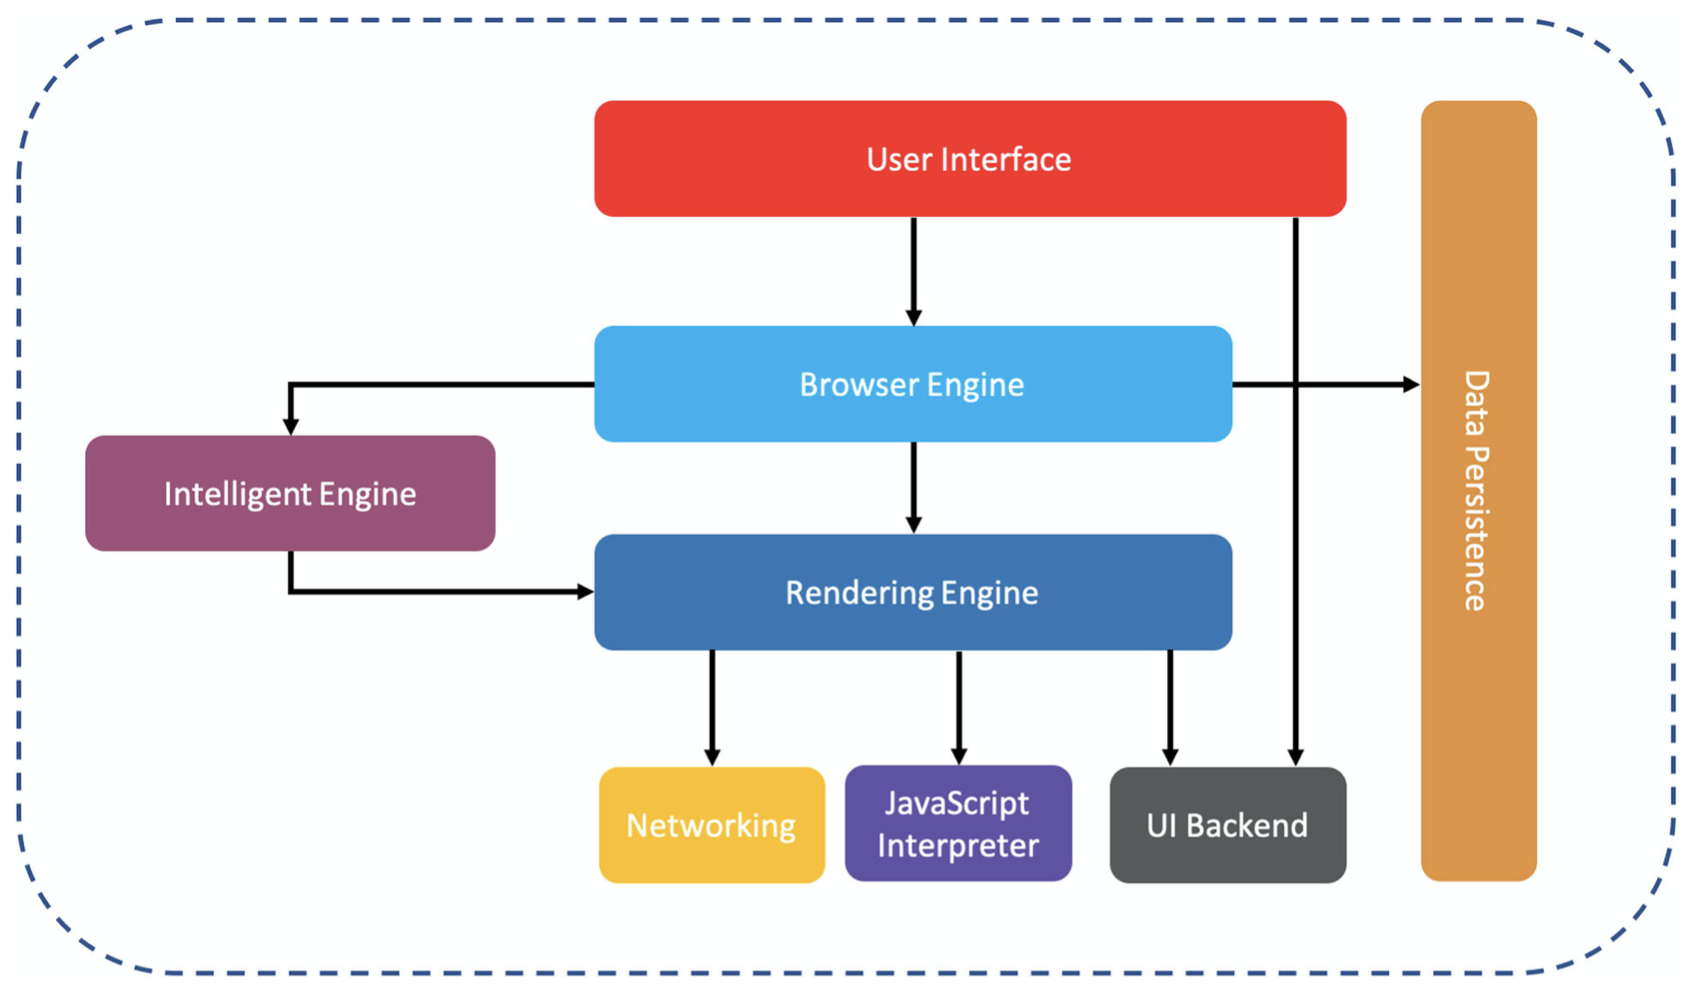
\includegraphics[width=0.8\linewidth]{images/EPDB_scheme.png}
    \caption{EPDB scheme}
    \label{fig:EPDB scheme}
\end{figure}

The system extracts 30 features from the URL, which are used by the intelligent module to detect a fraudulent site. If a phishing site is detected, the user is notified through a popup, allowing them to either stop or continue browsing. In the case of a phishing site, the execution of JavaScript code is halted, which is not something current browsers typically do. The ML model is stored in a pickle file and can be easily updated and redistributed.

\subsection{Dataset and Model}
To create the intelligent system, data from PhishTank and MillerSmiles were used. The dataset includes 11,055 records, with each record consisting of 30 features associated with the URL, allowing for the differentiation between fraudulent and safe websites.

The ML model employed to build the intelligent system is the Random Forest, an ensemble model of decision trees. Decision trees are easily interpretable, making it straightforward to understand which characteristics of a URL lead to its classification. However, these models are prone to overfitting, meaning they may adapt too closely to the training data and struggle to generalize effectively. To address this issue and achieve optimal performance, the authors used GridSearchCV to find the best model hyperparameters.

For training, the K-fold cross-validation technique was used. This involves performing K, in this case K=5, iterations where the dataset is divided into partitions (training and test), and the model is trained on these. The process is repeated K times, and an average of the model's performance is obtained.

It is interesting to see which features contributed the most to identifying fraudulent sites versus safe ones. The following graph highlights the most significant features in the case of the Random Forest model.

\begin{figure}[htp]
    \centering
    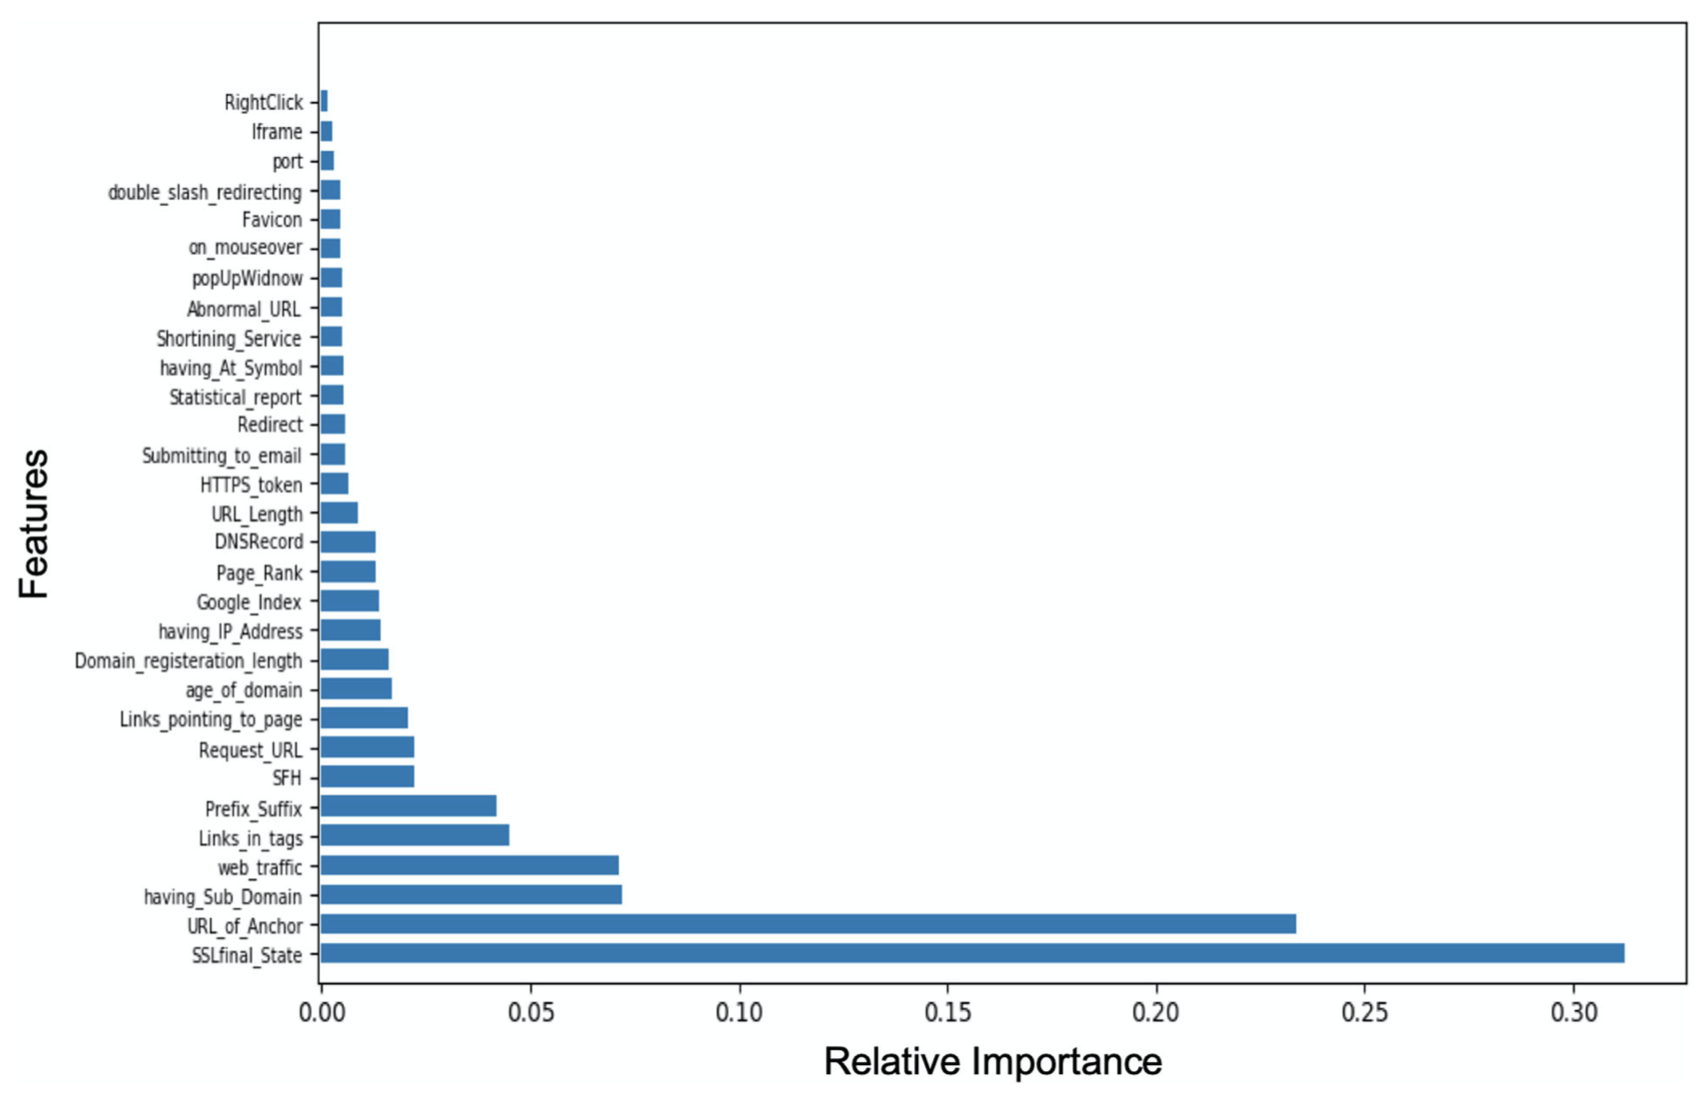
\includegraphics[width=1\linewidth]{images/30features_importance.png}
    \caption{Model-Based feature importance of 30 features}
    \label{fig:Relative importance of features}
\end{figure}
The 5 most important features are as follows:

\begin{enumerate}
    \item \textbf{SSLfinal\_State}: 
         This feature refers to the state of the site's SSL/TLS certificate. A valid and up-to-date SSL certificate is a signal of authenticity and security. In contrast, the lack of a certificate or the presence of an expired certificate could indicate a malicious site. 
         It is the most important feature because many phishing sites do not invest in proper SSL certificates or use short-lived certificates to avoid detection.
    
    \item \textbf{URL\_of\_Anchor}:
         This feature considers the percentage of links within the page that point to external domains compared to those that point to the same domain. A high number of outbound links can be indicative of phishing, as legitimate sites tend to have consistent internal links.
    
    \item \textbf{having\_Sub\_Domain}:
        This feature evaluates the presence and number of subdomains in the URL. A high number of subdomains or the use of unusual subdomains can be an indicator of a phishing site.
        Phishing attacks often use subdomains to mask suspicious URLs, making the URL appear similar to that of a legitimate site.
    
    \item \textbf{web\_traffic}:
        This feature analyzes the website's traffic using webpage rank. Sites with low traffic can be suspicious, as a legitimate site tends to have consistent and significant traffic.
        A phishing site usually has low web traffic since it is not regularly visited by normal users, but only by the victims of the attack.
    
    \item \textbf{Links\_in\_tags}:
        This feature measures the percentage of links within HTML tags (such as \texttt{<a>}, \texttt{<script>}, \texttt{<link>}, etc.). Phishers might insert malicious links into these tags to redirect users to phishing sites.
        A high percentage of links within these tags can be a direct indicator of a phishing attempt.
\end{enumerate}

The chart clearly shows that not all features contribute equally to the classification of a URL as benign or malicious. Some features, such as \textbf{RightClick} or \textbf{iframe}, have very low relative importance, indicating they are not strong indicators of phishing. In contrast, \textbf{SSLfinal\_State} and \textbf{URL\_of\_Anchor} are among the most important features, suggesting that the presence of a valid SSL certificate and the structure of the links within the site are key factors in determining the legitimacy of a site.

\subsection{Models Evaluations}
To determine the most suitable ML model for this task, SVM and Logistic Regression were also trained. The best model turned out to be the Random Forest, with an accuracy of 99.36\% and an F1-score of 99.43\%. The figure shows the confusion matrices for the three models mentioned.

\begin{figure}[htp]
    \centering
    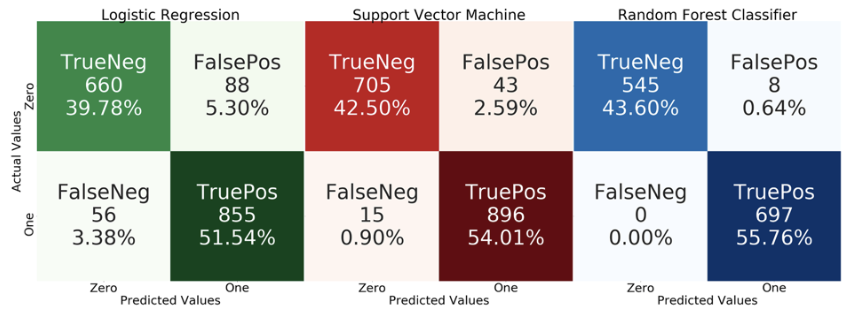
\includegraphics[width=1\linewidth]{images/ML_comparison.png}
    \caption{Confusion Matrix of ML models}
    \label{fig:Confusion Matrix of ML models}
\end{figure}

Another experiment focused on performance in terms of execution time. On average, the EPDB model was able to analyze a site in 4 seconds compared to 6 seconds for the Chrome extension, making this client-side solution more efficient.

\section{Phishing Detection with Generative Adversarial Network}

\subsection{System Overview}
The authors of this solution also adopted a completely URL-based approach, without considering the page content or third-party services. The system is structured as a \textbf{GAN}, which involves two Artificial Neural Networks (ANN) trained in an adversarial manner. Specifically, there is a generator, composed of a Long Short-Term Memory (LSTM) network, responsible for generating synthetic URLs (both fraudulent and legitimate). The discriminator, on the other hand, is a CNN tasked with analyzing the URL and classifying it as either legitimate or phishing.

The generator is trained to maximize the error made by the discriminator in recognizing the URL as synthetic, which indicates that it is improving in generating artificial URLs. Meanwhile, the discriminator is trained to recognize the generated URLs as accurately as possible, hence the term "adversarial neural networks."

Below is the structure proposed by the authors.

\begin{figure}[htp]
    \centering
    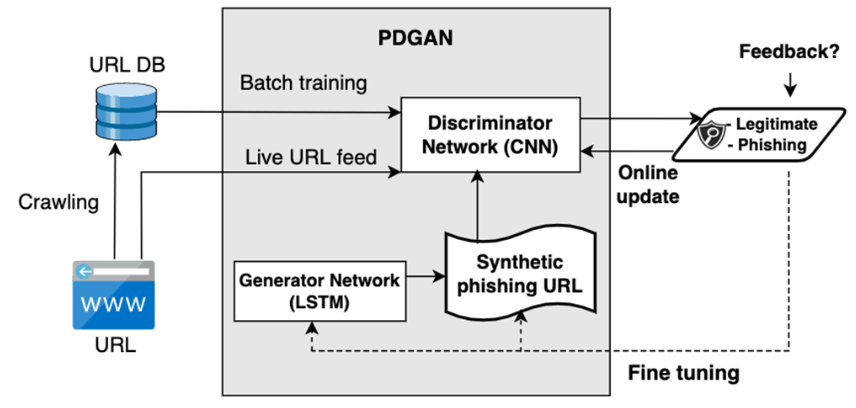
\includegraphics[width=0.8\linewidth]{images/PDGAN system.png}
    \caption{PDGAN Workflow}
    \label{fig:PDGAN Workflow}
\end{figure}

\subsection{Dataset and Model}
In this case as well, the dataset used comes from PhishTank, specifically MUPD, a balanced collection of 4.5 million URLs. After preprocessing (removing duplicates and balancing), the dataset is reduced to 2.3 million URLs. The preprocessed dataset is then randomly split into 60\% training, 20\% validation, and 20\% test sets. Since it is a balanced dataset, accuracy can be used as a metric to evaluate performance.

URLs cannot be directly fed into the model as plain text, so further preprocessing of the dataset is required to train the model. Specifically, it is assumed that the URL length does not exceed 255 characters, in accordance with the RFC2616 protocol. If it exceeds this limit, the URL is truncated; if it is shorter, zero padding is applied. Considering an alphabet of 69 characters (letters, numbers, and special characters), a one-hot vector is generated for each character in the URL, with a value of 1 corresponding to the represented character and all other characters set to 0, as shown in the figure.

\begin{figure}[htp]
    \centering
    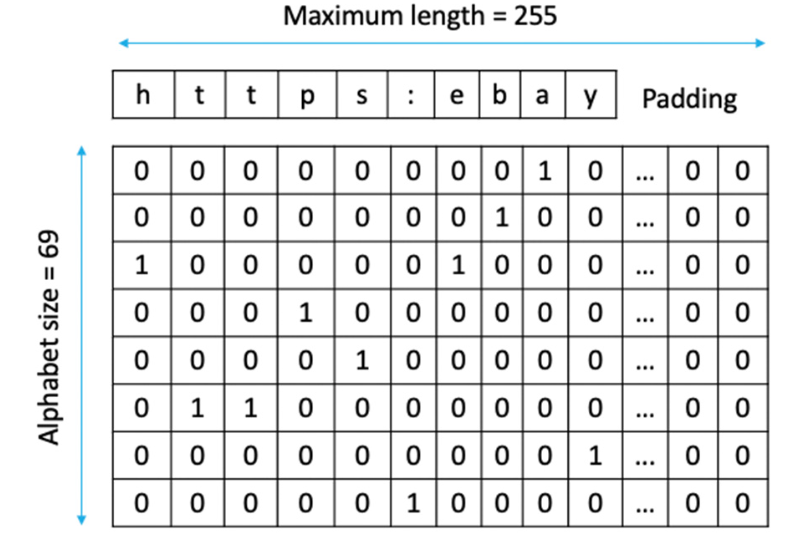
\includegraphics[width=0.8\linewidth]{images/URLs_preprocessing.png}
    \caption{URLs encording}
    \label{fig:URLs encording}
\end{figure}

This process is repeated for all URLs, and at this point, the dataset is ready to be used in the GAN.

\subsubsection{Generator}
The generator, as previously mentioned, is an LSTM, a type of network well-suited for storing long sequences of information. The structure of these networks consists of a set of memory cells connected to each other. Each cell has three main gates: the forget gate, the input gate, and the output gate. These gates regulate the flow of information into and out of the cell, enabling the LSTM to maintain and update its internal state over time.

\begin{figure}[htp]
    \centering
    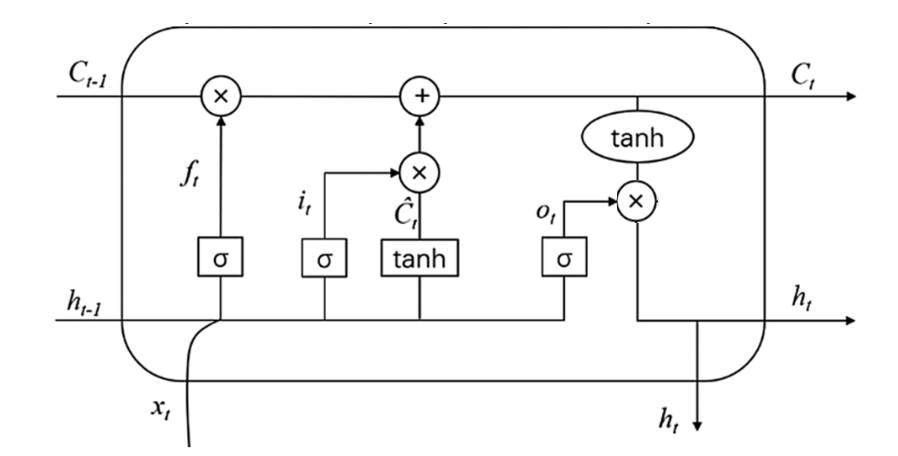
\includegraphics[width=0.8\linewidth]{images/generator_structure1.png}
    \caption{LSTM Cell}
    \label{fig:LSTM Cell}
\end{figure}

\textbf{Forget Gate}: The forget gate decides what information from the previous cell state \(C_{t-1}\) should be discarded. It outputs a value between 0 and 1 for each number in the cell state \(C_{t-1}\), where 1 represents "completely keep this" and 0 represents "completely forget this."
\[f_t = \sigma(W_f*[h_{t-1},x_t] + b_f)\]

\textbf{Input Gate}: The input gate determines which values from the input \(x_t\) will be used to update the cell state. It controls how much of the new input \(x_t\) should be added to the current cell state. 
\[i_t = \sigma(W_i*[h_{t-1},x_t] + b_i)\]

\textbf{Cell State Update}: The cell state \(C_t\) is then updated by combining the previous cell state \(C_{t-1}\) and the new candidate values \(\tilde{C}_t\) (scaled by the forget gate \(f_t\) and the input gate \(i_t\) respectively).
\[
C_t = f_t \otimes C_{t-1} \oplus i_t \otimes \tanh(W_c \cdot [h_{t-1}, x_t] + b_c)
\]

\textbf{Output Gate}: The output gate determines what the next hidden state \(h_t\) should be. This hidden state \(h_t\) is also used as the output of the LSTM cell. The output is based on the current cell state \(C_t\), passed through a \(\tanh\) function, and modulated by the output gate.
\[o_t = \sigma(W_o*[h_{t-1},x_t] + b_o)\]

In these equations, \(x_t\) is the input to the current layer, \(\sigma\) is the sigmoid function, \(h_{t-1}\) represents the hidden state at time \(t-1\), and \(b\) represents the bias for each gate. \(W_f\), \(W_i\), and \(W_o\) are the weight matrices for the connections.

Finally, the output of the LSTM cell, \(h_t\), is computed by combining the output gate \(o_t\) with the updated cell state \(C_t\), scaled through a \(\tanh\) function.
\[
h_t = o_t \otimes \tanh(C_t)
\]

\begin{figure}[htp]
    \centering
    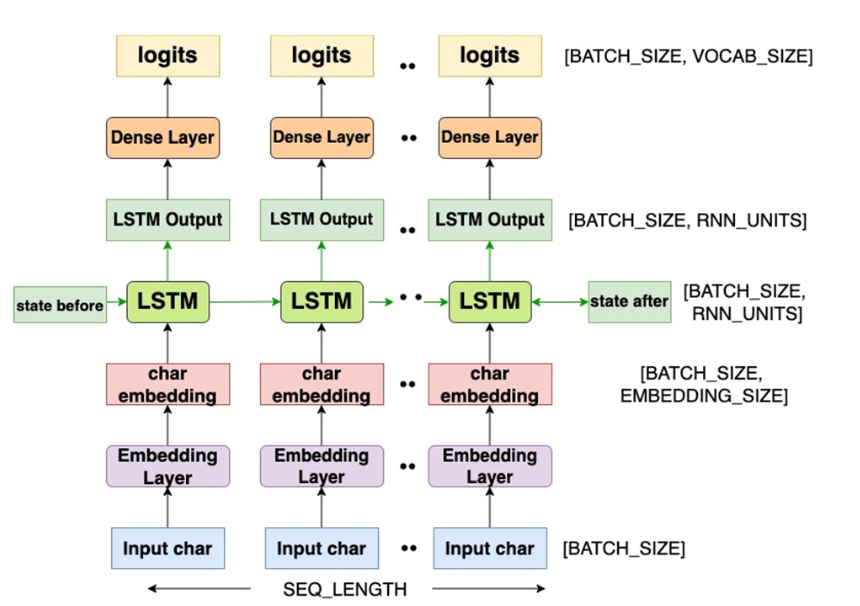
\includegraphics[width=0.8\linewidth]{images/generator_structure2.png}
    \caption{Generator architecture}
    \label{fig:Generator architecture}
\end{figure}

\subsubsection{Discriminator}
The discriminator is a CNN consisting of 9 layers in depth, with 6 convolutional layers and 3 fully connected dense layers. One-dimensional filters were used, which are convolutional filters that move in only one direction. Max-pooling layers were employed to extract the most relevant features and reduce the dimensionality, and dropout layers were used to decrease the number of network parameters, thereby reducing the likelihood of overfitting.

\subsubsection{DPGAN parameters}
For both models, binary cross-entropy was used as the loss function, with a learning rate of \textbf{0.001} and the Adam optimizer. The best results were achieved with \textbf{256} hidden layers and a batch size of \textbf{64} for the generator, at epoch 80. As for the discriminator, training was stopped at the twentieth epoch, and the best results were obtained using a convolutional kernel size of \textbf{{7,7,3,3,3,3}} and a batch size of \textbf{128}.

\subsection{Models Evaluations}
The authors compared their model with other similar models in the literature, specifically deep learning models that are URL-based and use the same dataset. Notably, PUCNN employs a CNN to extract character-level feature representations of URLs, while PDRCNN is based on a two-dimensional URL representation. It uses a biLSTM network to extract the global features of the constructed tensor and a CNN to extract the local features. 

\begin{figure}[htp]
    \centering
    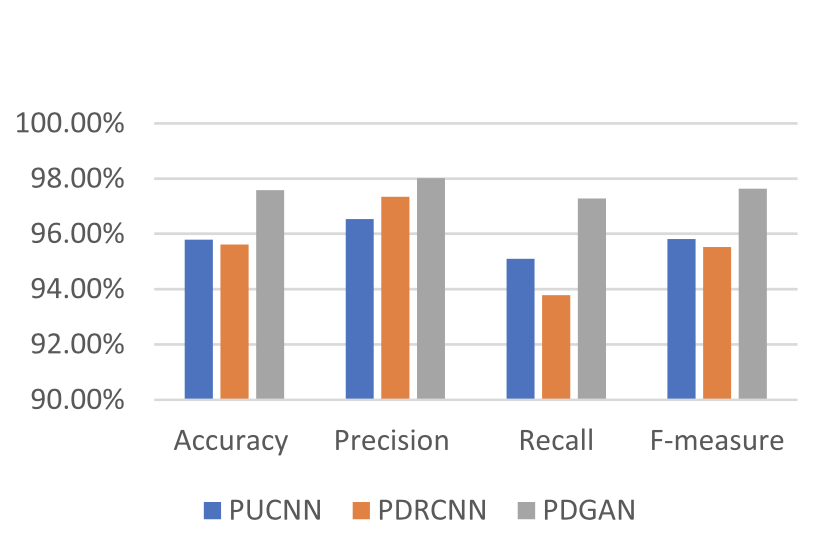
\includegraphics[width=0.8\linewidth]{images/DPGAN comparisongraph.png}
    \caption{DPGAN and Baselines comparison}
    \label{fig:DPGAN and Baselines comparison}
\end{figure}

The graph shows the results, highlighting that the DPGAN model achieved 98.02\% precision and 97.58\% accuracy, benefiting from the data augmentation provided by the generator.

\section{Phishing Detection using Transformer}

\subsection{System Overview}
The authors of this model propose a hybrid approach that combines URL-based analysis with partial content analysis of the web page to prevent the phishing attacks mentioned at the beginning of the document (BITB, Watering Hole, Clickjacking). Specifically, they suggest analyzing the URLs contained within the HTML and JavaScript code of the page in question to avoid the issue of embedding malicious code in legitimate content. This approach, therefore, strikes a balance between a purely URL-based approach (which is very fast but less accurate) and a content-based approach that analyzes the HTML, JavaScript, CSS, and DOM (which is much more accurate but also more complex and slower).

As shown in the figure, the system consists of a scraping and preprocessing phase. The collected data is then passed to a CNN, which extracts local features, followed by a Transformer encoder that encodes and identifies long-range dependencies among the various encodings to accurately classify the URL.

\begin{figure}[htp]
    \centering
    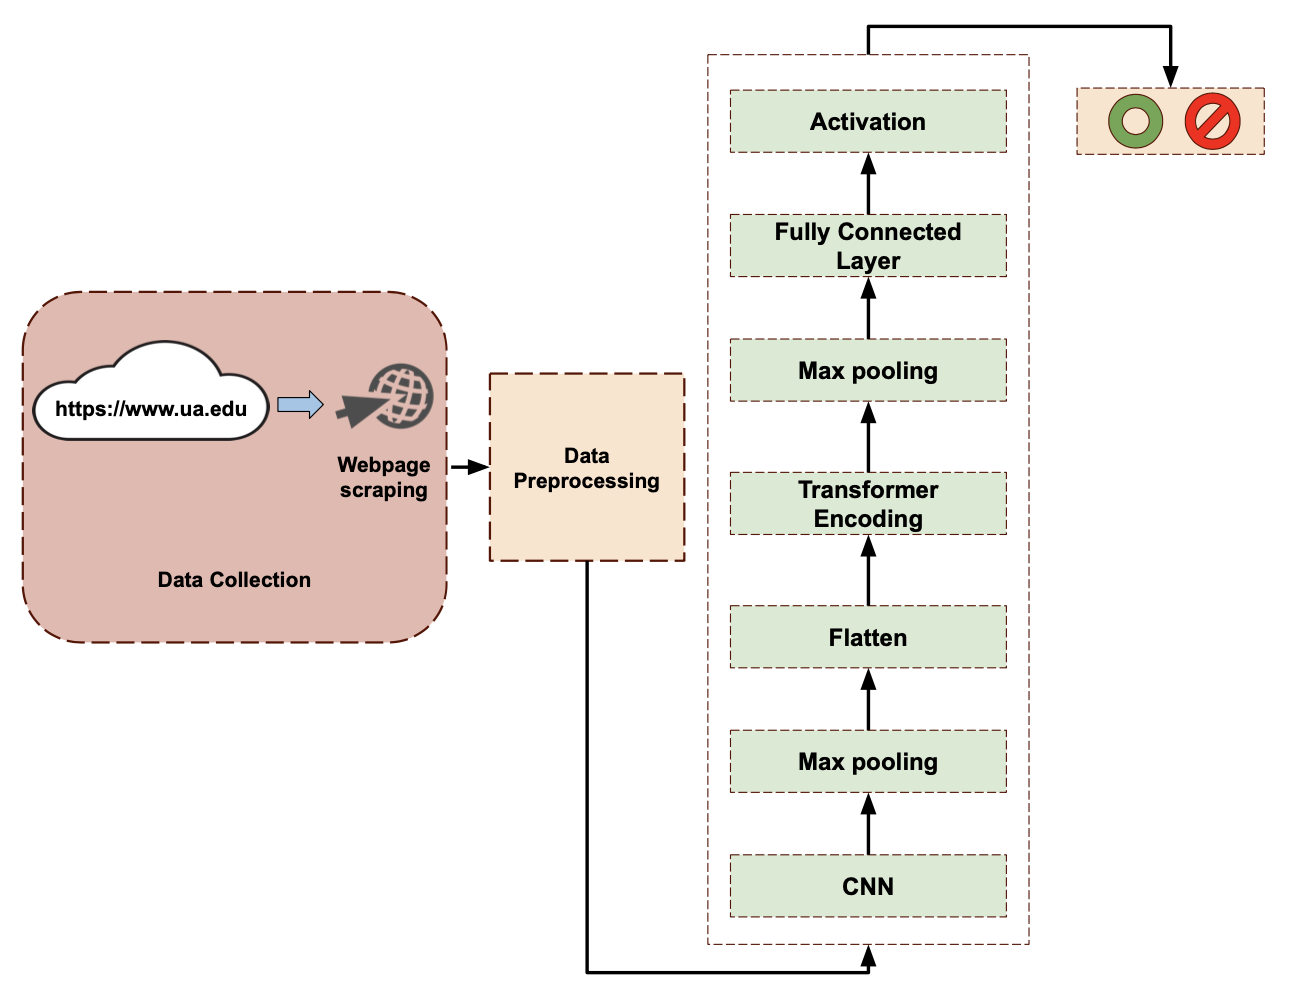
\includegraphics[width=0.8\linewidth]{images/transformer schema.png}
    \caption{CNN+Transformer schema}
    \label{fig:CNN+Transformer schema}
\end{figure}

\subsection{Dataset and Model}
The dataset consists of a collection of 50,000 malicious URLs from Phishtank and PhishArmy and a collection of 50,000 benign URLs from Alexa. For each URL, the online presence of the webpage was verified; if the page was not accessible, the URL was removed. If the page was accessible, web scraping was performed on the URL to retrieve all the URLs within the webpage, creating a list associated with the original URL \(X_i\) in the form \(X_i = [u_1,u_2,...,u_m]\). Thus, the final dataset is a matrix of the type \(D = [X_1,X_2,...,X_n]\).

The balanced dataset was partitioned into 70\% training, 20\% test, and 10\% validation.
\subsubsection{Preprocessing}
The preprocessing phase is quite important and consists of data scraping, cleaning, tokenization, and concatenation. Half of the URLs were found to be offline, so the final dataset consists of 50,000 URLs balanced between the classes. For tokenization, the authors use character-level tokenization, which allows the handling of unknown words. The possible characters considered include 92 options, including letters, numbers, and special characters. Additionally, four indices are introduced: `<PAD>` for padding, `<UNK>` for unknown characters, `<STA>` to mark the start of a URL, and `<SEP>` to mark the end of a URL.

The URL takes the form \(u = [c_1,c_2,...,c_d]\), with \(d\) being the fixed length of the URL. If a URL is longer than \(d\), it is truncated; if it is shorter, padding characters `<PAD>` are added. The same approach is applied to the lists of URLs contained within the target URL. If the list exceeds the limit of URLs per page, the excess URLs are removed; otherwise, padding URLs of the form `[<STA>,<PAD>,...,<PAD>,<SEP>]` are added. 

To determine the maximum URL length and the maximum number of URLs per page, an analysis was conducted on the data by class to choose the appropriate parameters. On average, a benign page is 62 characters long and contains 114 URLs, while a malicious page is 56 characters long and has 11 embedded URLs. The maximum number of characters per URL was set to 100 to allow some margin for error, and the maximum number of embedded URLs was set to 100 to avoid favoring either class.
\begin{figure}[htp]
    \centering
    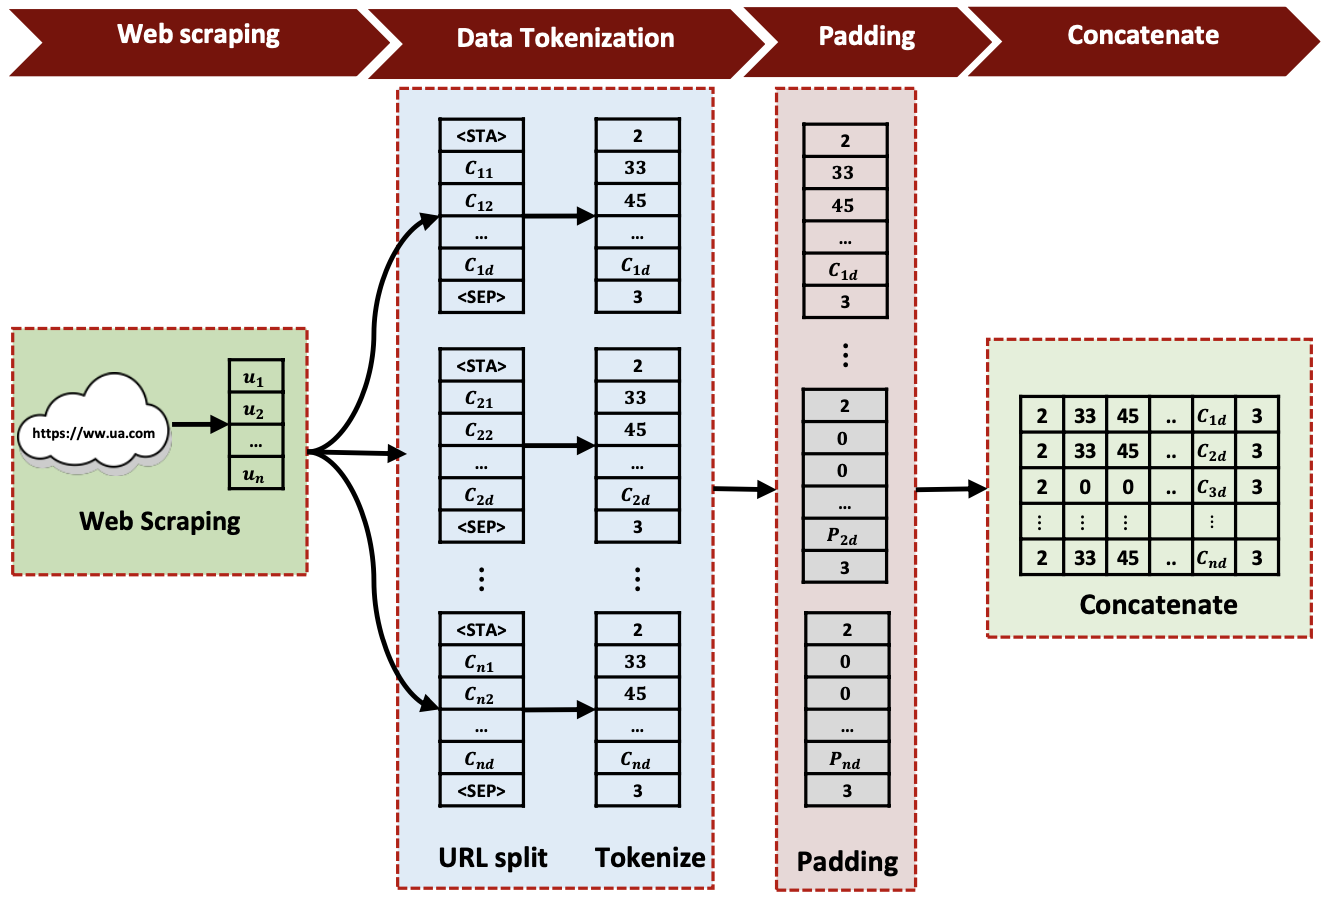
\includegraphics[width=0.8\linewidth]{images/transformer preprocessing.png}
    \caption{URL Preprocessing}
    \label{fig:URL Preprocessing}
\end{figure}

\subsubsection{Model structure}
The URLs constructed in this manner are then concatenated and are ready to be passed to the CNN. After this, a max pooling layer is applied to extract the most important features and significantly reduce the input space. A flatten layer is then used to convert the multi-dimensional array into a one-dimensional array, making it ready to be passed to the encoder.

The encoder is capable of capturing dependencies between the various symbols using the multi-head attention mechanism. Each character is associated with its position through a positional encoder. Then, each vector embedding is multiplied by three randomly initialized weights, called Query (Q), Key (K), and Value (V). The self-attention layer calculates a score for each character relative to the current character using the following formula:
\begin{equation}
Z(Q, K, V) = \text{softmax}\left(\frac{QK^T}{\sqrt{d_k}}\right)V
\end{equation}
Finally, a normalization layer is applied, which takes the self-attention output \(Z\) and the input \(X\) to stabilize the model's training. The encoder's output is passed through a max-pooling layer and then to a fully connected layer for classification.

\subsubsection{Model Parameters and Training}
The model was trained using K-fold cross-validation with \(k = 5\), and the hyperparameters used are shown in the figure below.

\begin{figure}[htp]
    \centering
    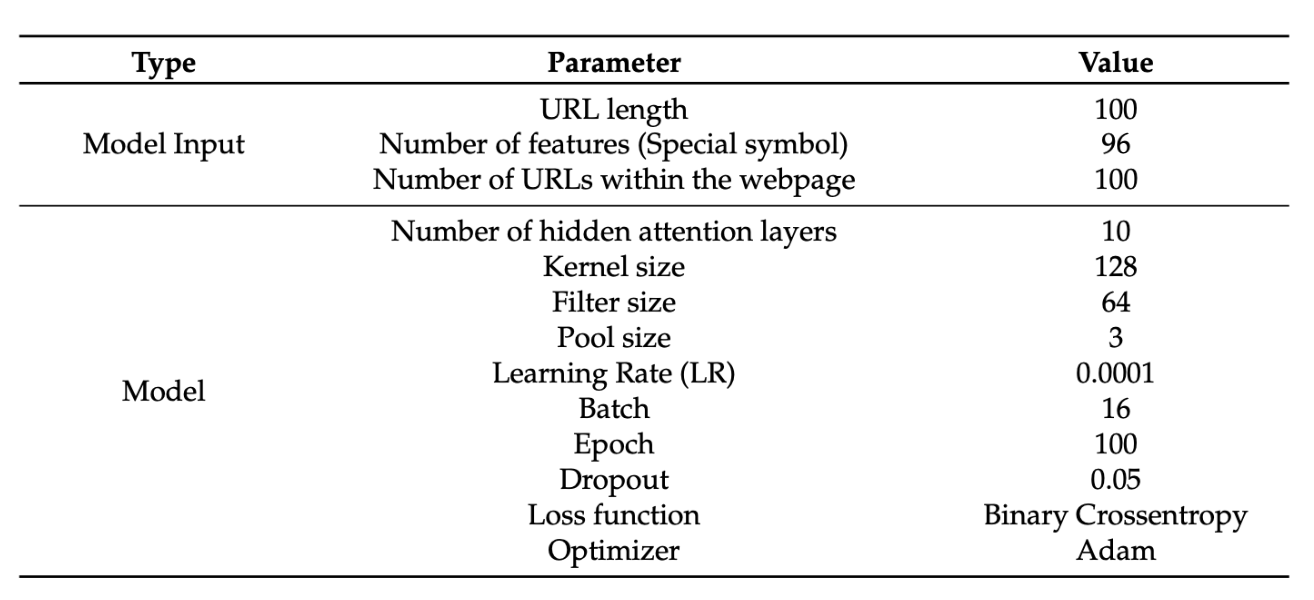
\includegraphics[width=1\linewidth]{images/Transformer parameters.png}
    \caption{CNN+Transformer parameters}
    \label{fig:CNN+Transformer parameters}
\end{figure}

\subsection{Models Evaluations}
 The generated model was compared with SVM, a CNN, and a biLSTM (which consists of two LSTMs—one processes the sequence from the first to the last element, and the other processes the sequence from the last to the first element). Additionally, two state-of-the-art models were considered as baseline models, both URL-based but differing in feature extraction and classification methods. URLNET is based on a CNN and performs feature extraction at three levels: character, word, and character-word. On the other hand, MPURNN is based on a biLSTM and focuses on character-level features.
\begin{figure}[htp]
    \centering
    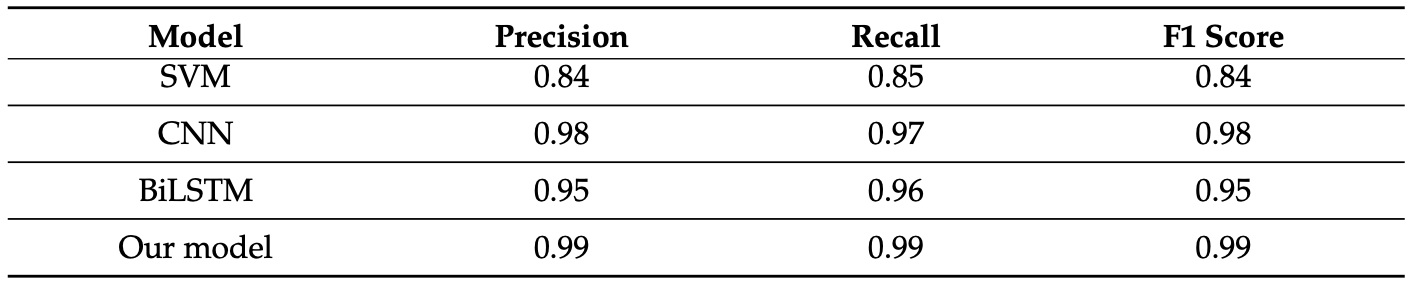
\includegraphics[width=1\linewidth]{images/TransformerComparison1.png}
    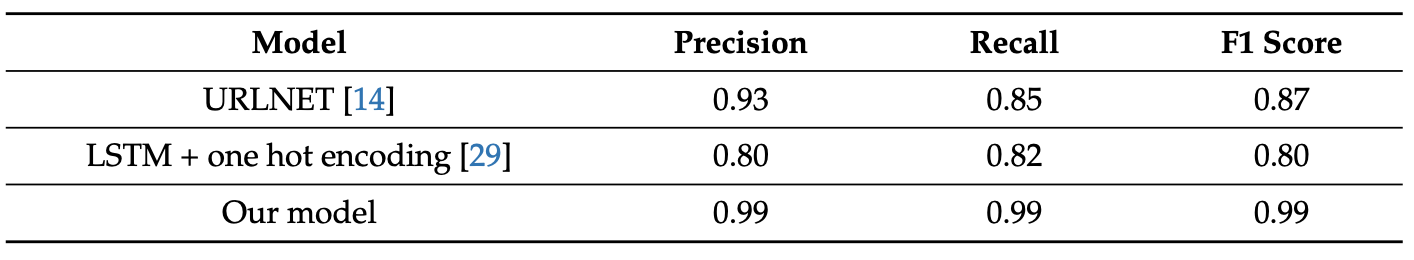
\includegraphics[width=1\linewidth]{images/TransformerComparison2.png}
    \caption{Models Comparison}
    \label{fig:Models Comparison}
\end{figure}
As we can see, in all cases, the model proposed by the authors outperforms the state-of-the-art models, achieving near-perfect performance with 99\% precision, recall, and F1-score.